\documentclass[tikz,border=3pt]{standalone}
\usepackage[utf8]{inputenc}
\usepackage[T1]{fontenc}
\usepackage{lmodern}
\renewcommand{\familydefault}{\sfdefault}
\usepackage{sansmath}\sansmath
\usepackage{chemfig}
\usepackage{pgfplots}\pgfplotsset{compat=1.18,/pgf/number format/use comma,/pgf/number format/1000 sep={.}}
\usetikzlibrary{arrows.meta,calc,positioning,decorations.pathmorphing,patterns}
% paleta del sitio
\definecolor{nar}{HTML}{E8680C}\definecolor{narc}{HTML}{FFB35C}\definecolor{hielo}{HTML}{FFF3E8}
\definecolor{tinta}{HTML}{1D1D1F}\definecolor{gris}{HTML}{6E6E73}\definecolor{lila}{HTML}{7C5CF0}
\definecolor{azul}{HTML}{2F6FD6}\definecolor{menta}{HTML}{17A673}\definecolor{coral}{HTML}{E8342A}
\tikzset{num/.style={circle,draw=tinta,fill=white,inner sep=1.5pt,font=\small\bfseries,text=tinta}}
\begin{document}
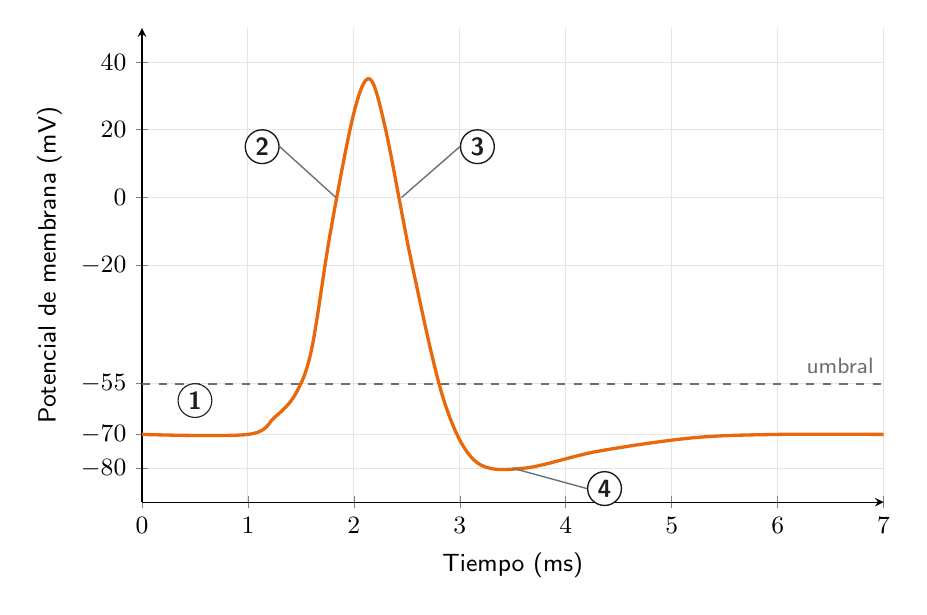
\begin{tikzpicture}[font=\small]
\begin{axis}[axis lines=left,grid=major,grid style={gray!20},xlabel={Tiempo (ms)},ylabel={Potencial de membrana (mV)},
  width=11cm,height=7.6cm,xmin=0,xmax=7,ymin=-90,ymax=50,ytick={-80,-70,-55,-20,0,20,40},xtick={0,1,...,7},clip=false]
\addplot[gris,dashed,thick,domain=0:7] {-55};
\addplot[nar,very thick,smooth,tension=0.55] coordinates {(0,-70)(1,-70)(1.25,-65)(1.45,-58)(1.6,-45)(1.78,-10)(2.0,25)(2.15,35)(2.3,20)(2.55,-20)(2.85,-60)(3.15,-78)(3.6,-80)(4.3,-75)(5.2,-71)(6,-70)(7,-70)};
\node[anchor=south east,text=gris,font=\footnotesize] at (axis cs:7,-55) {umbral};
\node[num] at (axis cs:0.5,-60) {1};
\draw[gris,line width=0.5pt] (axis cs:1.83,0) -- (axis cs:1.3,15) node[num,anchor=east] {2};
\draw[gris,line width=0.5pt] (axis cs:2.45,0) -- (axis cs:3.0,15) node[num,anchor=west] {3};
\draw[gris,line width=0.5pt] (axis cs:3.5,-80) -- (axis cs:4.2,-86) node[num,anchor=west] {4};
\end{axis}
\end{tikzpicture}
\end{document}
